\chapter{Materiais e Métodos}\label{cap:ferramentas}

Com o objetivo de obter melhor entendimento sobre possíveis ferramenta de visão computacional e detecção facial, este trabalho descreve a execução de testes utilizando a linguagem de programação Python e a implementa da ferramenta OpenCV \citeonline{itseez2015opencv} na mesma linguagem.

\section{OpenCV}

A ferramenta OpenCV \citeonline{itseez2015opencv} é uma biblioteca de código aberto focada em problemas de visão computacional em tempo real, desenvolvida pela intel e posteriormente pela Itseez, com suporte a múltiplas plataformas e uso gratuito sobre a licença de código aberto BSD. A ferramenta apresenta suporte a frameworks de aprendizado profundo, como TensorFlow, Pytorch e Caffe \citeonline{wiki:OpenCV} e contempla tanto funções básicas, para aplicações como processamento de imagem, alteração de cor ou resolução, até aplicações avançadas, como detecção facial, identificação de características e biometria.

Neste trabalho, será utilizada a função de detecção de faces da ferramenta OpenCV, que utiliza um classificador em cascata baseado características, este é um método eficiente para reconhecimento de faces em imagens proposto por Paul Viola and Michael Jones, amplamente conhecido como método Viola-Jones, onde uma função é treinada com muitos exemplos positivos (imagens que contém o objeto a ser detectado) e negativos (imagens que não contém o objeto a ser detectado) e então utilizada para detectar as mesmas características em outras imagens. \cite{itseez2014theopencv}

A detecção de faces utilizando OpenCV consiste em duas etapas principais, o treinamento do modelo, onde são apresentadas diversas imagens já identificadas para que o modelo identifique padrões positivos e negativos. Após o treinamento, o modelo obtido pode ser utilizado para identificar, em novas imagens, características semelhantes as vistas nas imagens do treinamento. Neste projeto, será utilizado um modelo fornecido em conjunto com a ferramenta OpenCV, já treinado com diversos exemplos de faces frontais.

\section{Algoritmo Viola-Jones}

O algoritmo Viola-Jones foi publicado em 2001, no paper "Rapid object detection using a boosted cascade of simple features" ~\cite{paper-viola-jones} e é famoso por sua capacidade de detecção de faces com muita velocidade, isso ocorre devido a 3 principais técnicas utilizadas: o cálculo da imagem integral, o algoritmo de impulsão \textit{AdaBoost} e o classificador em cascata.

%-
\subsection{Imagem Integral}
%-

A primeira etapa do algoritmo Viola-Jones consiste em transformar a imagem original em uma imagem integral, isto é feito calculando o valor de cada pixel como a soma de todos os pixels que estão acima ou a esquerda do mesmo, como ilustrado na figura~\ref{fig:integral}.

\begin{figure}[htpb]
    \centering
    \caption{Imagem original (esquerda) e imagem integral (direita).}
    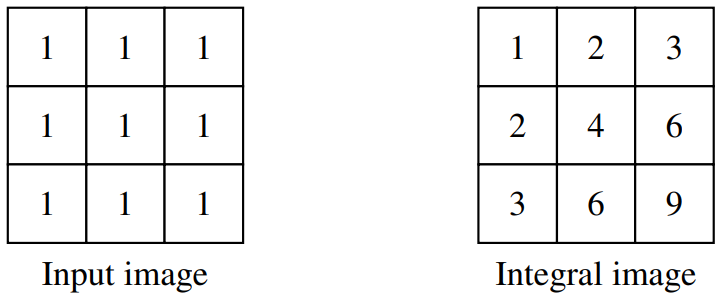
\includegraphics[scale=.3]{figs/imagem-integral.png}
    \legend{Fonte: \citeauthoronline{jensen2008implementingviolajones} (\citeyear{jensen2008implementingviolajones})}
    \label{fig:integral}
 \end{figure}

A utilização desta técnica permite calcular facilmente o tamanho de qualquer retângulo formado entre quatro pixels da imagem, conhecendo apenas o valor dos seus cantos, possibilitando assim a análise rápida de diversas partes da imagem. Tal calculo é feito definindo o retângulo a ser análisado e então aplicando a equação \ref{eq:img-integral}.

\begin{figure}[htb]
    \centering
    \caption{Representação da área da imagem a ser analisada.}
    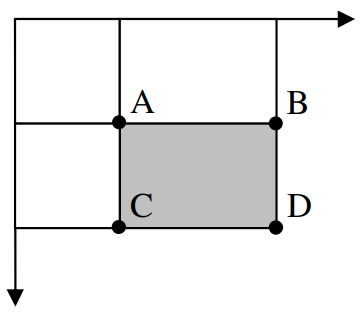
\includegraphics[scale=.3]{figs/imagem-integral-calculo.png}
    \legend{Fonte: \citeauthoronline{jensen2008implementingviolajones} (\citeyear{jensen2008implementingviolajones})}
    \label{fig:integral-calculo}
 \end{figure}

 \begin{equation}\label{eq:img-integral}
    \text{ Soma do retângulo cinza } = D - (B + C) + A
\end{equation}

Com a possibilidade de calcular facilmente a soma dos pixels de um retângulo arbitrário de forma rápida, o algoritmo para detecção pode analisar diversos trechos da imagem, chamados aqui de características, fazendo a comparação de duas ou mais áreas retângulares predefinidas, como os exemplos ilustrado na figura \ref{fig:features}. 

\begin{figure}[htb]
    \centering
    \caption{Alguns exemplos de características retângulares analisadas.}
    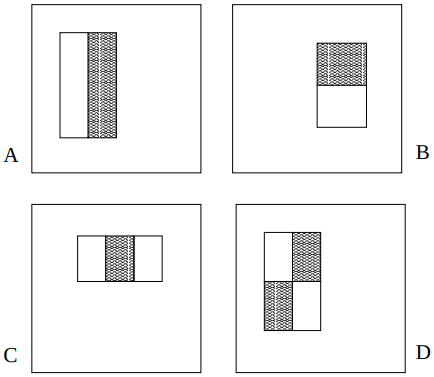
\includegraphics[scale=.3]{figs/features.png}
    \legend{Fonte: \citeauthoronline{paper-viola-jones} (\citeyear{paper-viola-jones})}
    \label{fig:features}
 \end{figure}

 O valor final de cada característica é definido pela soma do valor dos pixels sob o retângulo cinza menos a soma do valor dos pixels sob o retângulo branco.

%-
\subsection{Algoritmo de Impulsão AdaBoost}
%-

As características demonstradas anteriormente, são definidas basicamente como duas ou mais áreas retângulares de qualquer tamanho, tal simplicidade implica na possibilidade da criação de uma enorme variação das mesmas que precisariam ser calculadas diversas vezes, para cada parte de imagem e com diferentes tamanhos, isso implica em um alto custo de processamento, para evitar tal problema, durante a etapa de treinamento do modelo, é utilizado o algoritmo de impulsão \textit{AdaBoost}, que identifica quais são as características com maior probabilidade de acerto.

O \textit{AdaBoost}, que tem seu nome derivado de \textit{adaptative boosting} \citeonline{fabio-luciana-2015} (traduzido como impulsão adaptativa), é um método de aprendizado de máquina que utiliza a combinação de vários classificadores fracos para obter uma classificação forte, no caso da detecção facial, o algoritmo é utilizado tanto para selecionar um conjunto de características mais eficientes como para treinar o classificador.

\begin{figure}[htb]
    \centering
    \caption{Características retângulares mais eficientes para detecção facial.}
    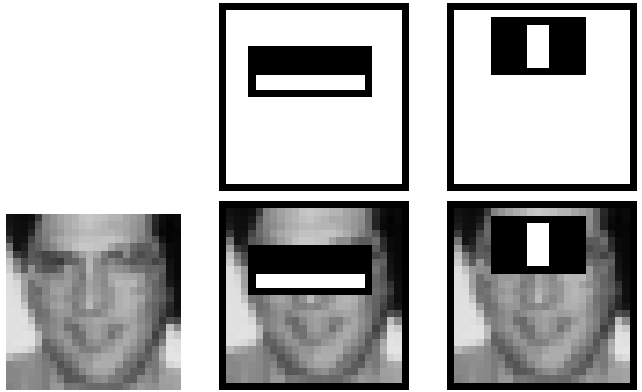
\includegraphics[scale=.3]{figs/top-features.png}
    \legend{Fonte: \citeauthoronline{paper-viola-jones} (\citeyear{paper-viola-jones})}
    \label{fig:top-features}
 \end{figure}

 A figura \ref{fig:top-features} retrata as melhores características registradas por \citeauthoronline{paper-viola-jones} (\citeyear{paper-viola-jones}), fica claro que as mesmas se destacam por evidenciar as regiões dos olhos e do nariz.

%-
\subsection{Classificador em Cascata}
%-

Pensando que, na maioria dos casos, uma face não ocupa a maior parte de uma imagem a ser identificada, é necessário encontrar uma forma rápida de descartar os elementos do fundo da mesma e concentrar o poder de processamento nos elementos que tem maior probabilidade de serem reconhecidos como uma face, isso leva a uma formulação para o problema onde ao contrário de encontrar faces, é necessário um algoritmo que descarte as "não faces".

Para tal problema, o classificador em cascata apresenta uma ótima solução, esta consiste na utilização de uma série de classificadores que são aplicados de forma sequencial, conforme ilustrado na imagem \ref{fig:cascade-classifier}, permitindo que imagens que certamente não possuem faces sejam rapidamente descartadas logo nas primeiras iterações, enquanto imagens com possíveis faces são classificadas por toda cascata, trazendo um elevado nível de confiança ao resultado.

\begin{figure}[htb]
    \centering
    \caption{Diagrama do funcionamento do classificador em cascata.}
    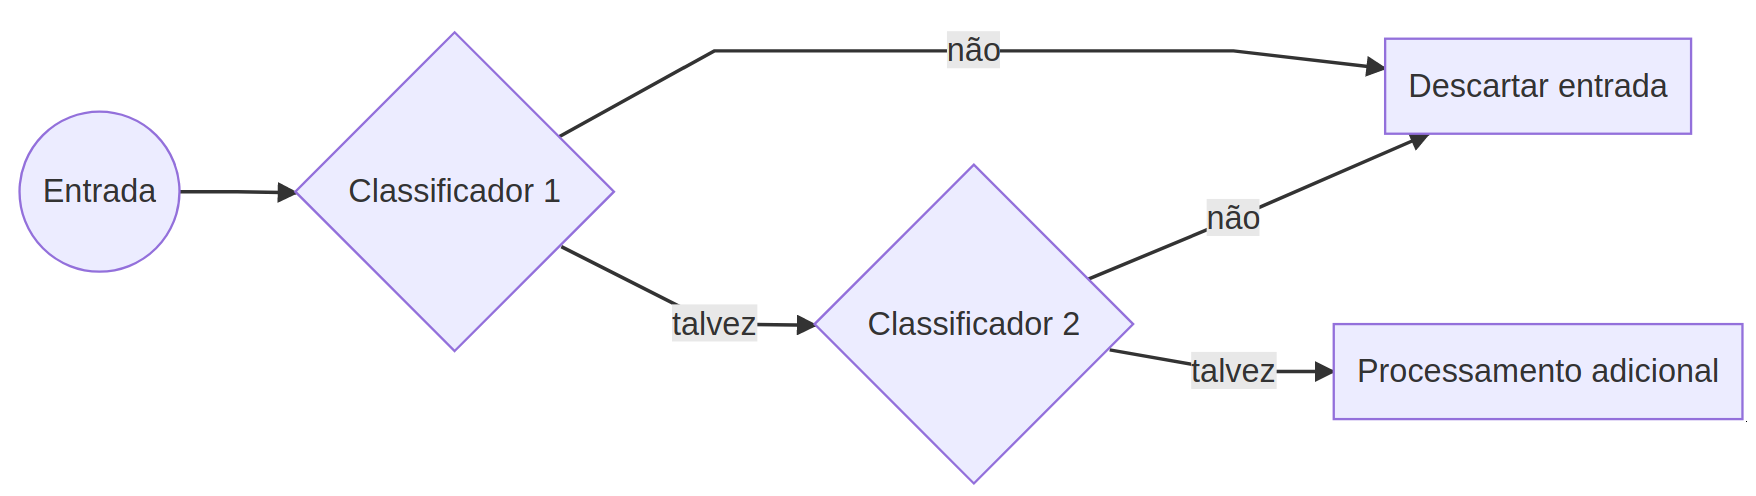
\includegraphics[scale=.3]{figs/cascade-classifier.png}
    \legend{Fonte: \citeauthoronline{paper-viola-jones} (\citeyear{paper-viola-jones})}
    \label{fig:cascade-classifier}
 \end{figure}

 Um classificador comum, com um único estágio normalmente aceitaria muitos casos de falso negativo, para reduzir a taxa de falsos positivos e de descarte de imagens relevantes, mas no classificador em cascata, falsos positivos nos primeiros estágios não são um problema, pois serão analisados em outros diversos estágios e provavelmente eliminados.

 A utilização desse modelo combinada com o algoritmo \textit{AdaBoost}, possibilita a análise das característica mais eficientes logo no início e consequentemente o descarte muito mais rápido dos casos negativos nos primeiros estágios.
